\section{Design of the LNA}

\subsection{Transistor Bias Network}

The DC bias point of a transistor directly influences its small-signal S-parameters, and hence the gain, noise figure and stability of the LNA. This makes this step crucial.
Figure \ref{fig:DCBiasNPN} shows the biasing circuit and its Thévenin equivalent used to simplify analysis.

\begin{figure}[H]
    \centering
    \begin{subfigure}{0.4\textwidth}
        \includegraphics*[scale = 0.3]{Images/DCBiasNPN.png}
        \caption{Transistor DC biasing circuit.}
    \end{subfigure}
    \hfill
    \begin{subfigure}{0.4\textwidth}
        \includegraphics*[scale = 0.3]{Images/VthBiasCircuit.png}
        \caption{Bias circuit equivalent circuit.}
        \label{fig:DCBiasTh}
    \end{subfigure}
    \caption{Transistor DC biasing circuit and its Thévenin equivalent.}
    \label{fig:DCBiasNPN}
\end{figure}

As shown in Figure \ref{fig:DCBiasTh} the Thévenin equivalent is given by the equations \ref{eq:biasThev}, replacing the $R_1$, $R_2$ voltage divider.

\begin{equation}
    \begin{split}
        R_{TH} &= R_1//R_2\\
        V_{TH} &= V_{cc}\frac{R_2}{R_1+R_2}
    \end{split}
    \label{eq:biasThev}
\end{equation}

Using Kirchhoff voltage law, the equations \ref{eq:biasKVL} are derived, the first starts at $V_{TH}$ goes through $R_{TH}$, $V_{BE}$ and $R_4$. The second goes from $V_{CC}$ through $R_3$, $V_{CE}$ and $R_4$. 

\begin{equation}
    \begin{cases}        
        0 = V_{TH} -I_b\cdot R_{TH} - V_{BE}-I_E\cdot R_4  \\
        0 = V_{CC} - R_3\cdot I_C - V_{CE} - I_E \cdot R_4\\
    \end{cases}
    \label{eq:biasKVL}
\end{equation}

Solving the system of equations, assuming fixed values for $R_2$ and $R_4$, originates the equations \ref{eq:biasr1r3}.

\begin{equation}
    \begin{split}
        R_1 &= \frac{R_{2} \left(- I_{C} R_{4} \beta - I_{C} R_{4} - V_{BE} \beta + V_ {CC} \beta\right)}{I_{C} R_{2} + I_{C} R_{4} \beta + I_{C} R_{4} + V_{BE} \beta}\\
        R_3 &= \frac{- I_{C} R_{4} \beta - I_{C} R_{4} + V_{CC} \beta - V_{CE} \beta}{I_{C} \beta}
    \end{split}
    \label{eq:biasr1r3}
\end{equation}

The Table \ref{tab:BiasParam}, shows the provided values for the biasing circuit and the fixed values for $R_2$ and $R_4$.

\begin{table}[h]
    \centering
    \caption{Transistor biasing parameters}
    \begin{tabularx}{\textwidth}{>{\centering\arraybackslash}X >{\centering\arraybackslash}X}
        \toprule
        \textbf{Parameter} & \textbf{Value} \\
        \midrule
        $R_2$     & $1\,\si{\kilo\ohm}$ \\
        \midrule
        $R_4$     & $100\,\si{\ohm}$\\
        \midrule
        $\beta$   & $72.534$ \\
        \midrule
        $I_C$     & $9\,\si{\milli\ampere}$ \\
        \midrule
        $V_{CC}$  & $10\,\si{\volt}$ \\
        \midrule
        $V_{BE}$  & $1\,\si{\volt}$ \\
        \midrule
        $V_{CE}$  & $\SI{5}{\volt}$\\
        \bottomrule
    \end{tabularx}
    \label{tab:BiasParam}
\end{table}

Resulting in $R_1 = \SI{4}{\kilo\ohm}$ and $R_3 = \SI{454}{\ohm}$.

\subsection{S-parameters with packaging effects}

The diagram of the LNA is shown in Figure \ref{fig:LNA-diagram}, where the LNA has arbitrary input and output impedances different from $50\,\si{\ohm}$ and reflection coefficients.

\begin{figure}[H]
    \centering
    \includegraphics[width=0.8\textwidth]{Images/LNA-diagram-no-match.png}
    \caption{LNA diagram with reflection coefficients and no matching networks.}
    \label{fig:LNA-diagram}
\end{figure}

With the biasing circuit designed, the next step was to simulate the S-parameters of the transistor in LTSpice.  The S-parameters were taken for a frequency range of $1\,\si{\giga\hertz}$ to $10\,\si{\giga\hertz}$, Figure \ref{fig:withoutmathing} shows the S-parameters of the transistor without any matching network.

\begin{figure}[H]
    \centering
    \includegraphics[width=0.6\textwidth]{Images/without-matching.png}
    \caption{S-parameters of the transistor, for the range of frequencies, without matching network.}
    \label{fig:withoutmathing}
\end{figure}


\subsection{Stability}


Ensuring that the LNA remains stable is critical for reliable operation. The network is unconditionally stable for a frequency if for any source impedance value, $|\rho_{in}|<1$  and for the load impedance $|\rho_{out}|<1$.
Below, the stability analysis is performed using the S-parameters obtained in the previous step to calculate the stability factors, ins this case, the $K$ and $\Delta$ factors and the $\mu$ factor.

Defining $\Delta$ as:

\begin{equation}
    \Delta = S_{11}\cdot S_{22} - S_{12}\cdot S_{21}
    \label{eq:Delta}
\end{equation}

Where $S_{11}$, $S_{22}$, $S_{12}$ and $S_{21}$ are the S-parameters of the LNA. 

And defining $K$ as:

\begin{equation}
    K = \frac{1-|S_{11}|^2-|S_{22}|^2+|\Delta|^2}{2|S_{12}\cdot S_{21}|}
\end{equation}

The stability conditions can be summarized as follows:

\begin{itemize}
    \item $K>1$ and $|\Delta|<1\rightarrow$ unconditionally stable
    \item $K>1$ and $|\Delta| > 1$ or  $K<1 \rightarrow$ potentially unstable or always unstable
\end{itemize}

Another criteria is the $\mu$ factor, defining $\mu$ as:

$$\mu = \frac{1-|S_{11}|^2}{|S_{22}-\Delta S_{11}^*| + |S_{12}\cdot S_{21}|}$$

If $\mu > 1\rightarrow$ unconditionally stable
In addition, it can be said that larger values of $\mu$ imply greater stability.

\begin{figure}[H]
    \centering
    \includegraphics[width=0.6\textwidth]{Images/KFactor.png}
    \caption{Stability factors $K$, $\Delta$ and $\mu$ for the range of frequencies.}
    \label{fig:StabilityTest}
\end{figure}

Figure \ref{fig:StabilityTest}, shows that the LNA is stable for frequencies above $\SI{3.1}{\giga\hertz}$ and above $\SI{10}{\giga\hertz}$ loses stability again.

At this stage another important figure is the Maximum Available Gain, $MAG$, which for the bilateral case can be expressed as the equation \ref{eq:MAG}.

\begin{equation}
    MAG = \left | \frac{S_{21}}{S_{12}} \right |\cdot \left[ K - \sqrt{K^2-1} \right]
    \label{eq:MAG}
\end{equation}

\begin{figure}[H]
    \centering
    \includegraphics[width=0.6\textwidth]{Images/MAG.png}
    \caption{Maximum Available Gain for the range of frequencies.}  
    \label{fig:MAG}
\end{figure}

Now having the full picture of the LNA characteristics, an operating frequency can be decided. 
The frequency chosen was the one that maximizes the gain while maintaining stability. In this case, the chosen was $\SI{4}{\giga\hertz}$, where the $MAG$ is $26,13$ and the stability factors are $K=1,05$, $\Delta=0,35$ and $\mu=1,06$, the summary of the stability parameters is shown in Table \ref{tab:StabilityParam}.

\begin{table}[h]
    \centering
    \caption{Stability parameters for the chosen frequency.}
    \begin{tabularx}{\textwidth}{>{\centering\arraybackslash}X >{\centering\arraybackslash}X}
        \toprule
        \textbf{Parameter} & \textbf{Value} \\
        \midrule
        Chosen Frequency     & $4\,\si{\giga\hertz}$ \\
        \midrule
        $|\Delta|$     & $0,35$\\
        \midrule
        $k$   & $1,05$ \\
        \midrule
        $\mu$     & $1,06$ \\
        \midrule
        $MAG$  & $26,13$ \\
        \bottomrule
    \end{tabularx}
    \label{tab:StabilityParam}
\end{table}

The stability circles in the Smith Chart for the input and output are shown in Figure \ref{fig:StabilityCircles}, where is possible to see  that at $4\si{\giga\hertz}$ the LNA is stable for all the source and load impedances.

\begin{figure}[H]
    \centering
    \includegraphics[width=0.6\textwidth]{Images/stability-circles.png}
    \caption{Stability circles for the input and output of the LNA.}
    \label{fig:StabilityCircles}
\end{figure}

\subsection{Input and output matching networks for Maximum Gain}

The adaptation for maximum gain is done using the line impedance transformation method. The input and output matching networks are designed to transform the input and output impedances of the transistor to the desired values, which are $50\,\si{\ohm}$ in this case. In the Smith Chart, the matching is done with inductors and capacitors or lines and stubs.

In Figure \ref{fig:LNA-diagram} the diagram of the LNA is shown, where is possible to see the reflection coefficients, the input and output matching networks, the source and load impedances $Z_0$.

\begin{figure}[H]
    \centering
    \includegraphics[width=1\textwidth]{Images/LNA-diagram.png}
    \caption{LNA diagram with matching networks and reflection coefficients.}
    \label{fig:LNA-diagram}
\end{figure}

Observing the diagram, the input and output matching networks are designed to transform the input and output impedances of the transistor to $50\,\si{\ohm}$, corresponding to the source and load impedances $Z_0$.

The maximum power transfer from the input matching network to the transistor will occur when:

\begin{equation}
    \Gamma_{in} = \Gamma_{s}^*
    \label{eq:GammaS=GammaL}
\end{equation}

And the maximum power transfer from the transistor to the output matching network will occur when:
\begin{equation}
    \Gamma_{out} = \Gamma_{l}^*
    \label{eq:GammaL=GammaS}
\end{equation}
where $\Gamma_{in}$ and $\Gamma_{out}$ are the reflection coefficients at the input and output of the transistor, respectively, and $\Gamma_{s}$ and $\Gamma_{l}$ are the reflection coefficients at the source and load impedances, respectively. Using the equations obtain in \cite{Pozar}, the expression that result in the reflection coefficients at the input and output of the transistor are:

\begin{equation}
    B_1 = 1 + |S_{11}^2| - |S_{22}|^2 - |\Delta|^2 
    \label{eq:B1}
\end{equation}
\begin{equation}
    B_2 = 1 + |S_{22}^2| - |S_{11}|^2 - |\Delta|^2
    \label{eq:B2}
\end{equation}
\begin{equation}
    C_1 = S_{11} - \Delta S_{22}^*
    \label{eq:C1}
\end{equation}
\begin{equation}
    C_2 = S_{22} - \Delta S_{11}^* 
    \label{eq:C2}
\end{equation}

Finally, the reflection coefficients at the source and load of the transistor are given by:

\begin{equation}
    \Gamma_{S} = \frac{B_1 \pm \sqrt{B-1^2-4|C_1|^2}}{2C_1}
    \label{eq:GammaS}
\end{equation}

\begin{equation}
    \Gamma_{L} = \frac{B_2 \pm \sqrt{B-2^2-4|C_2|^2}}{2C_2}
    \label{eq:GammaL}
\end{equation}

In Table \ref{tab:ReflectionCoefficients} the reflection coefficients at the input and output of the transistor are shown, where the values are calculated using the S-parameters obtained in the previous step.
\begin{table}[H]
    \centering
    \caption{Reflection coefficients at the input and output of the transistor.}
    \begin{tabularx}{\textwidth}{>{\centering\arraybackslash}X >{\centering\arraybackslash}X}
        \toprule
        \textbf{Parameter} & \textbf{Value} \\
        \midrule
        $\Gamma_{S}$     & $-0.61339711-0.4649262j$ \\
        \midrule
        $\Gamma_{L}$     & $0.29177619+0.6148401j$\\
        \midrule
        $B_{1}$     & $1.03559444$\\
        \midrule
        $B_{2}$     & $0.72244362$\\
        \midrule
        $C_{1}$     & $-0.39891088+0.30235572j$\\
        \midrule
        $C_{2}$     & $0.144066-0.30358047j$\\
        \midrule
        $S_{11}$     & $-0.33990673+0.27537675j$\\
        \midrule
        $S_{12}$     & $0.06042986-0.17647029j$\\
        \midrule
        $S_{21}$     & $0.09296393+0.05839295j$\\
        \midrule
        $S_{22}$     & $2.52965222+2.95848991j$\\
        \bottomrule
    \end{tabularx}
    \label{tab:ReflectionCoefficients}
\end{table}

With the values of the reflection coefficients at the source and load, the normalized impedances at the source and load can be calculated using the equations \ref{eq:Zs} and \ref{eq:Zl}.

\begin{equation}
    z_{S} = \frac{1+\Gamma_{S}}{1-\Gamma_{S}}
    \label{eq:Zs}
\end{equation}
\begin{equation}
    z_{L} = \frac{1+\Gamma_{L}}{1-\Gamma_{L}}
    \label{eq:Zl}
\end{equation}

Where $Z_0$ is the desired impedance, in this case $50\,\si{\ohm}$.
The resulting normalized impedances at the source and load are shown in Table \ref{tab:Impedances}, where the values are calculated using the reflection coefficients obtained in the previous step.

\begin{table}[H]
    \centering
    \caption{Impedances at the source and load of the transistor.}
    \begin{tabularx}{\textwidth}{>{\centering\arraybackslash}X >{\centering\arraybackslash}X}
        \toprule
        \textbf{Parameter} & \textbf{Value} \\
        \midrule
        $z_{S}$     & $0.14457529-0.32982769j$ \\
        \midrule
        $z_{L}$     & $0.6103145+1.39798452j$\\
        \bottomrule
    \end{tabularx}
    \label{tab:Impedances}
\end{table}

The Smith Chart representation of the normalized impedances at the source and load is shown in Figure \ref{fig:ZsZl}, where the normalized impedances are represented as points.
\begin{figure}[H]
    \centering
    \includegraphics[width=0.6\textwidth]{Images/ZsZl-smithChart.png}
    \caption{Normalized impedances at the source and load of the transistor in the Smith Chart.}
    \label{fig:ZsZl}
\end{figure}



\subsubsection{Matching with lumped elements}

The matching networks were first designed using the Smith chart, which allows for the visualization of the impedance transformation. A second analysis was done with an analytic approach using a Python script in order to have more accurate results. The input and output impedances of the LNA are transformed to $50\,\si{\ohm}$ using a combination of inductors and capacitors. The values of the components are also calculated using the equations for impedance transformation. 

\vspace{0.4cm}
\textbf{Results with the Smith Chart:}
\vspace{0.4cm}

The matching using the Smith Chart for the input and output are shown in Figures \ref{fig:zs-LC-matching} and \ref{fig:zl-LC-matching}, where the input and output impedances of the transistor are transformed to $50\,\si{\ohm}$ using a combination of inductors and capacitors, in this case a L-section matching network.

\begin{figure}[H]
    \centering
    \includegraphics[width=0.6\textwidth]{Images/zs-lc-match.png}
    \caption{Smith chart for input matching with lumped elements.}
    \label{fig:zs-LC-matching}
\end{figure}

The adaptation mesh for the input was done with a shunt capacitor and a series inductor and the equivalent circuit is shown in Figure \ref{fig:MatchingCircuit-input}. The values of the components were also calculated using the equations for impedance transformation as a form of validation.

\begin{figure}[H]
    \centering
    \includegraphics[width=0.5\textwidth]{Images/Input-matching-circuit.png}
    \caption{Matching circuit for input.}
    \label{fig:MatchingCircuit-input}
\end{figure}

\begin{figure}[H]
    \centering
    \includegraphics[width=0.6\textwidth]{Images/zl-lc-match.png}
    \caption{Smith chart for output matching with lumped elements.}
    \label{fig:zl-LC-matching}
\end{figure}

The adaptation mesh for the output is done with a series inductor and a shunt inductor and the equivalent circuit is shown in Figure \ref{fig:MatchingCircuit-output}. The values of the components were also calculated using the equations for impedance transformation as a form of validation.

\begin{figure}[H]
    \centering
    \includegraphics[width=0.5\textwidth]{Images/Ouput-matching-circuit.png}
    \caption{Matching circuit for output.}
    \label{fig:MatchingCircuit-output} 
\end{figure}

After retrieving the values of the in-between impedances $Z_a$ from the Smith Chart, it is possible to obtain the values of the components using the following equations \textsuperscript{\cite{Pozar}}:

\vspace{0.4cm}
Series inductor:
\begin{equation}
    \begin{split}
        z_L = z_2 -  z_1 = jx \quad(x > 0)\\
        L = \frac{xZ_0}{\omega}
    \end{split}
    \label{eq:SeriesInductor}
\end{equation}

Shunt Inductor:
\begin{equation}
    \begin{split}
       y_L = y_2 -  y_1 = -jb \quad(b > 0)\\
        L = \frac{Z_0}{b\omega} 
    \end{split}
    \label{eq:ShuntInductor}
\end{equation}

Series Capacitor:
\begin{equation}
    \begin{split}
        z_C = z_2 -  z_1 = -jx \quad(x > 0)\\
        C = \frac{1}{xZ_0\omega}
    \end{split}
    \label{eq:SeriesCapacitor}
\end{equation}

Shunt Capacitor:
\begin{equation}
    \begin{split}
        y_C = y_2 -  y_1 = jb \quad(b > 0)\\
        C = \frac{b}{Z_0\omega}
    \end{split}
    \label{eq:ShuntCapacitor}
\end{equation}

\vspace{0.4cm}
From input in-between impedance $Z_a = 0,14-0,34j$ and the configuration chosen in the smith chart represented in Figure \ref{fig:MatchingCircuit-input}, the values of the components are calculated as follows:

\vspace{0.4cm}
Shunt Capacitor:
\begin{equation}
    \begin{split}
        y_C =y_a-y_0 = 1+2,5j - 1 = 2,5j\\
        b = 2,5 \\
        C_{in} = \frac{2,5}{2\pi410^9Z_0} = 1,989\,\si{\pico\farad}
    \end{split}
    \label{eq:InputCap}
\end{equation}

Series Inductor:
\begin{equation}
    \begin{split}
        z_L = z_s - z_a = 0,14-0,33j - 0.14 - 0,34j = 0,01j\\
        x = 0,01 \\
        L_{in} = \frac{0,01\cdot Z_0}{2\pi410^9} = 198,9\,\si{\femto\henry}
    \end{split}
    \label{eq:InputInd}
\end{equation}

From output in-between impedance $Z_a = 0,6+0,48j$ and the configuration chosen in the Smith Chart represented in Figure \ref{fig:MatchingCircuit-output}, the values of the components are calculated as follows:

\vspace{0.4cm}
Shunt Inductor:
\begin{equation}
    \begin{split}
        y_L = y_a - y_0 = 1-0.81- 1 = -0,81j\\
        b = 0,81 \\
        L_{1out} = \frac{Z_0}{0,81\cdot2\pi4\cdot10^9} = 2,46\,\si{\nano\henry}
    \end{split}
    \label{eq:OutputIndShunt}
\end{equation}

Series Inductor:
\begin{equation}
    \begin{split}
        z_L = z_l - z_a = 0,6 + 1,4j - 0,6 + 0,48 = 0,92j\\
        x = 0,92 \\
        L_{2out} = \frac{0,92\cdot Z_0}{2\pi4\cdot10^9} = 1,83\,\si{\nano\henry}
    \end{split}
    \label{eq:OutputInd}
\end{equation}

\vspace{0.4cm}
\textbf{Results with analytic approach:}
\vspace{0.4cm}

The matching using the analytic approach was done using a Python script (Appendix \ref{appendix:python_script}) that calculates the values of the components based on the input and output impedances of the transistor. The equations used in the script are the following\textsuperscript{\cite{Pozar}}:

Matching for z inside the $1+jx$ circle:

\begin{equation}
    B = \frac{x_l \pm \sqrt{rl/z_0}\sqrt{r_l^2 + x_l^2- z_0 r_l}}{r_l^2+ x_l^2}
\end{equation}

\begin{equation}
    X = \frac{1}{B}+\frac{x_l z_0}{r_l}-\frac{z_0}{Br_l}
\end{equation}

For this case the network is designed with a series reactance and a shunt suspectance, where $B$ is the component suspectance and $X$ the component reactance, as shown in Figure \ref{fig:inside-matching}.
\begin{figure}[H]
    \centering
    \includegraphics[width=0.5\textwidth]{Images/outside-matching.png}
    \caption{Matching circuit for z inside the $1+jx$ circle.}
    \label{fig:inside-matching}
\end{figure}

Matching for z outside the $1+jx$ circle:
\begin{equation}
    X = \pm \sqrt{r_l(z_0-r_l)}-x_l
\end{equation}

\begin{equation}
    B = \pm \frac{\sqrt{(z_0-rl)/r_l}}{z_0}
\end{equation}

For this case the network is designed with a shunt suspectance and a series reactance, as shown in Figure \ref{fig:outside-matching}.
\begin{figure}[H]
    \centering
    \includegraphics[width=0.5\textwidth]{Images/inside-matching.png}
    \caption{Matching circuit for z outside the $1+jx$ circle.}
    \label{fig:outside-matching}
\end{figure}

With $B$ being the component suspectance and $X$ the component reactance, $r_l$ the real part of the impedance $z$ and $x_l$ the imaginary part of the  normalized impedance $z$.

The results of the matching networks using the analytic approach are shown in Table \ref{tab:MatchingValues}, where the values of the components are calculated based on the input and output impedances of the transistor.

\begin{table}[H]
    \centering
    \caption{Values of the components for the matching networks using the analytic approach.}
    \begin{tabularx}{\textwidth}{>{\centering\arraybackslash}X >{\centering\arraybackslash}X}
        \toprule
        \textbf{Parameter} & \textbf{Value} \\
        \midrule
        $C_{in}$     & $1.93417775\,\si{\pico\farad}$ \\
        \midrule
        $L_{in}$     & $43.4243305\,\si{\pico\henry}$\\
        \midrule
        $L_{1out}$   & $2.4877816\,\si{\nano\henry}$ \\
        \midrule
        $L_{2out}$   & $1.8095882\,\si{\nano\henry}$\\
        \bottomrule
    \end{tabularx}
    \label{tab:MatchingValues}
\end{table}

Comparing the values obtained from the Smith Chart and the analytic approach, it is possible to see that the values are very similar, with a difference of less than $5\%$ in all cases. This validates the results obtained from the Smith Chart.

The resulting circuit, with the final values, is shown in Figure \ref{fig:MatchingCircuit}.
\begin{figure}[H]
    \centering
    \includegraphics[width=1\textwidth]{Images/LC_matching-circuit.png}
    \caption{Matching circuit for input and output with final values.}
    \label{fig:MatchingCircuit}
\end{figure}

\subsubsection{Matching lines and stubs}
The matching networks were also designed using transmission lines and stubs, this type of adaptation allows greater frequencies (more than 1 \si{\giga \hertz}) in real conditions. The input and output impedances of the transistor were transformed to $50\,\si{\ohm}$ using a combination of transmission lines and stubs. The values of the components were also calculated using the equations for impedance transformation to validate the results.

The matching using the Smith Chart for the input and output are shown in Figures \ref{fig:zs-line-matching} and \ref{fig:zl-line-matching}.

% \begin{figure}[H]
%     \centering
%     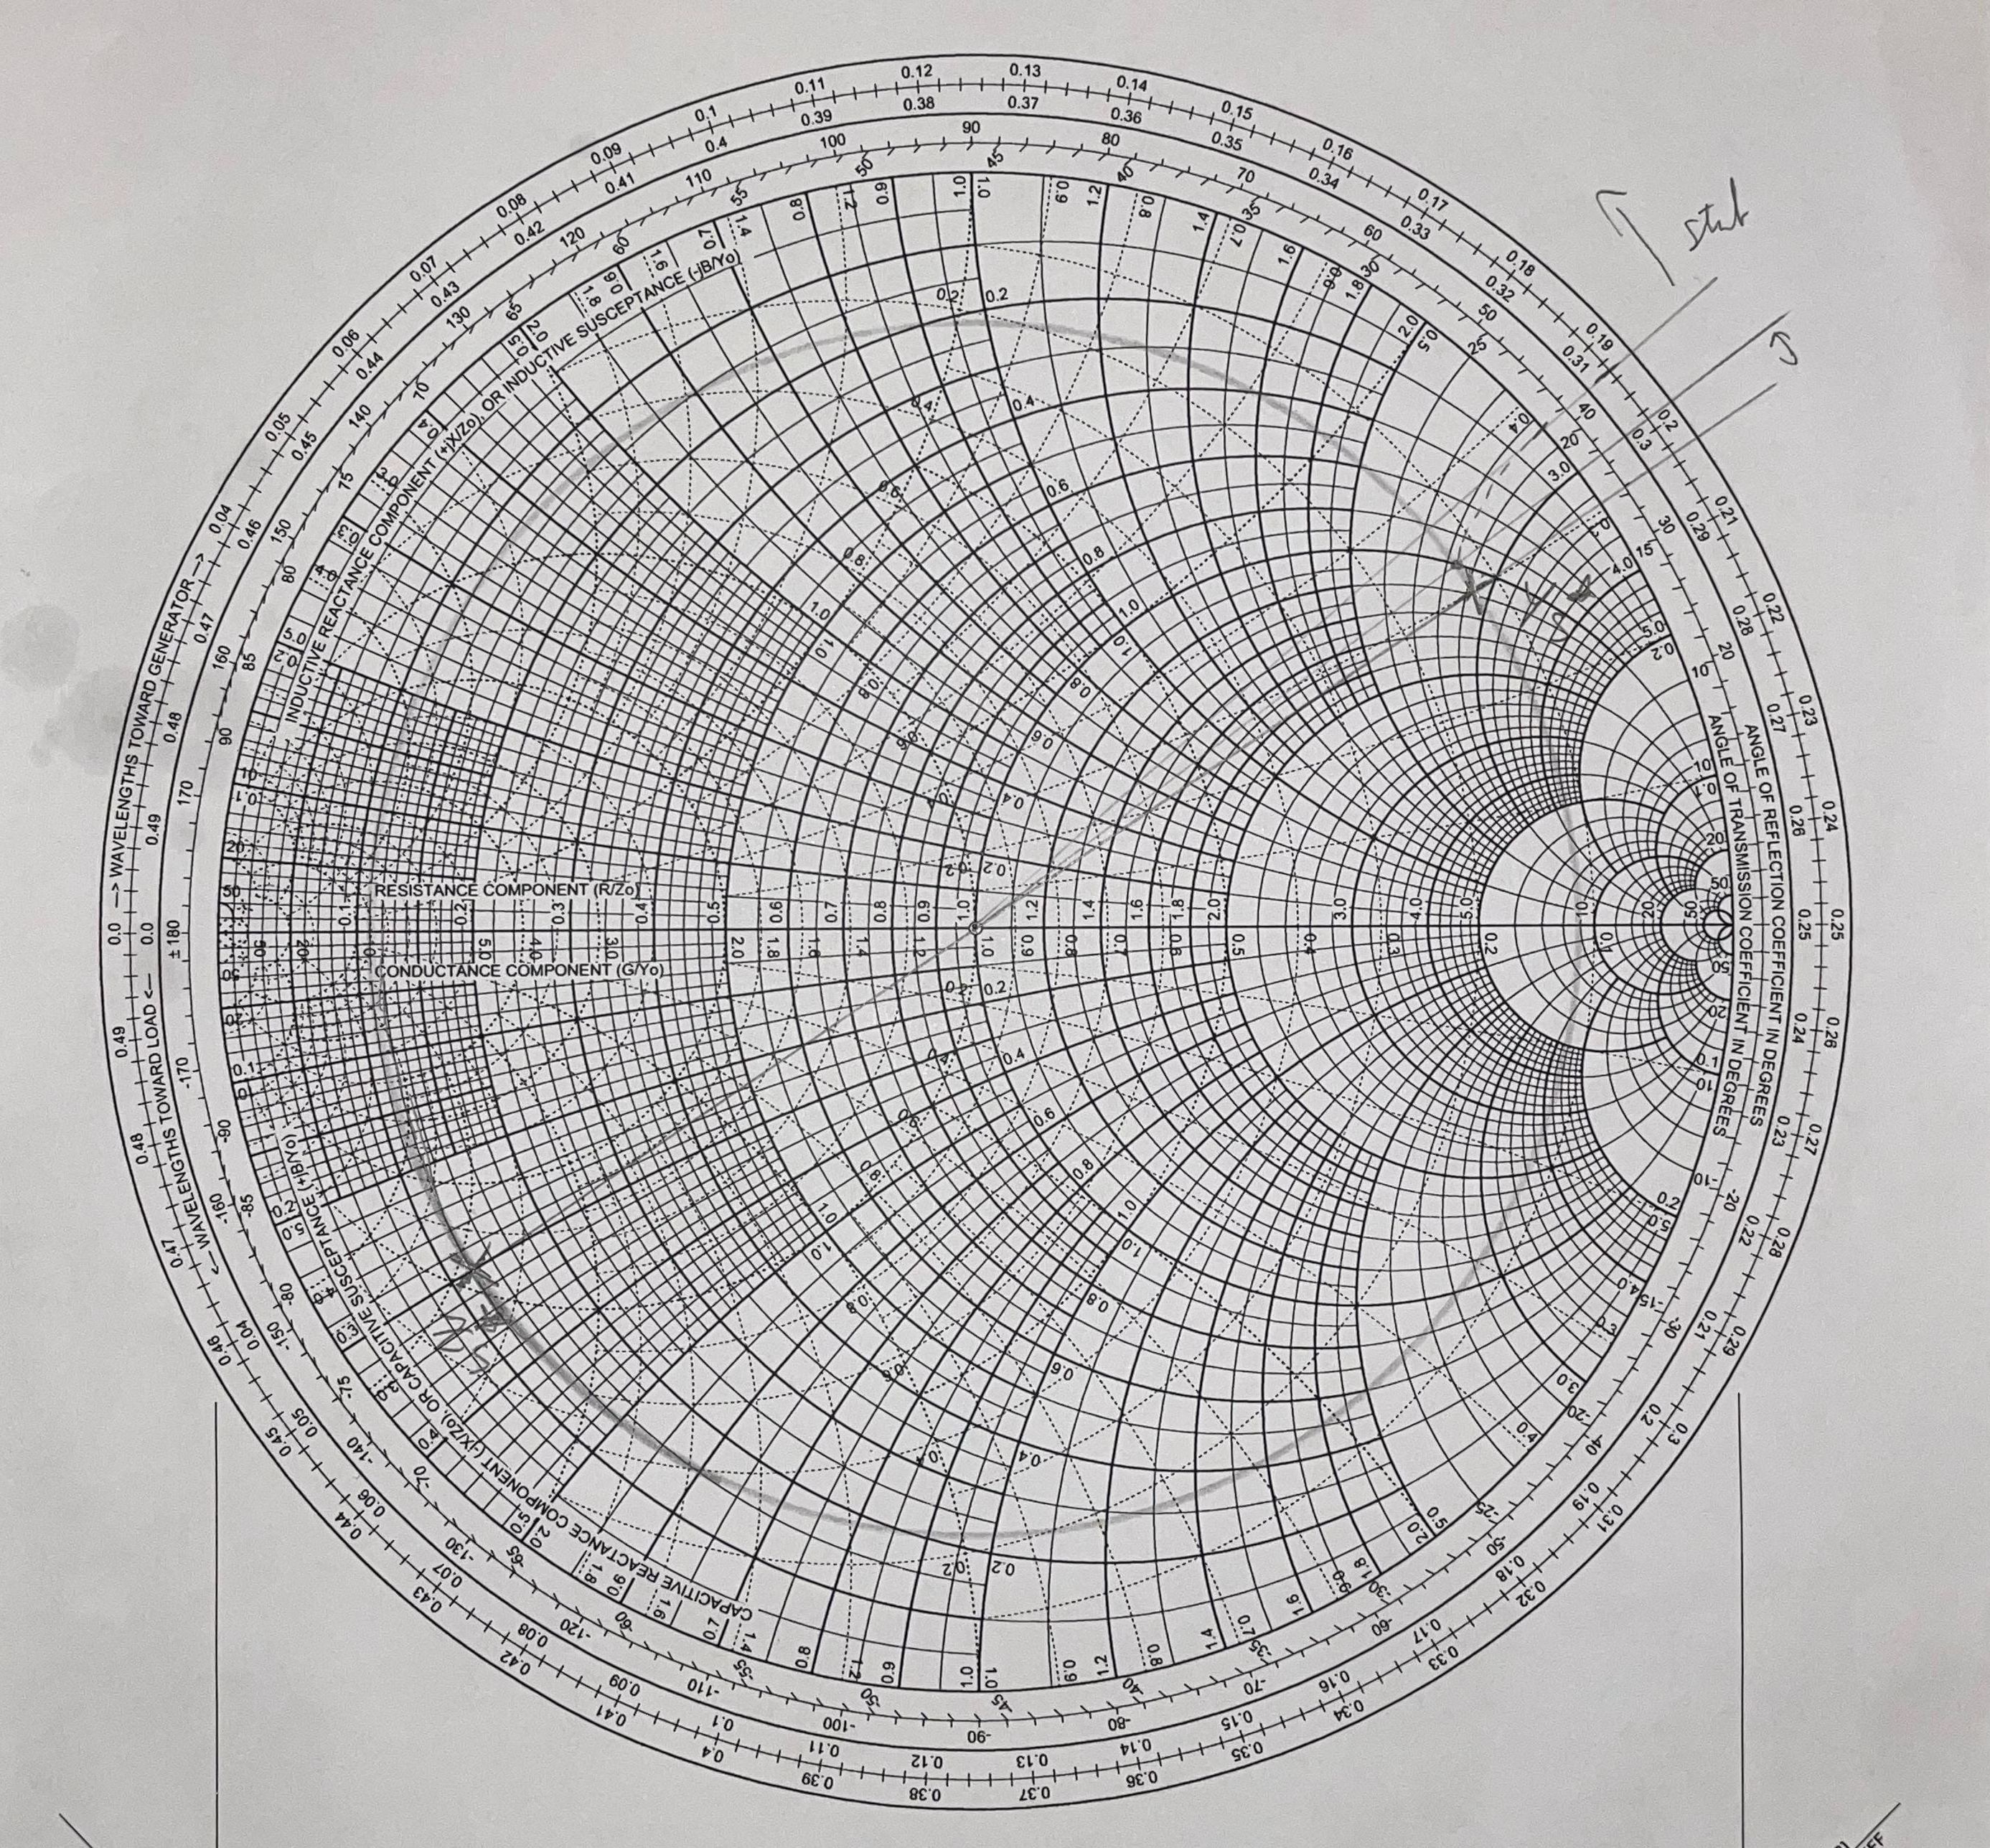
\includegraphics[width=0.5\textwidth]{Images/zs-LS-matching.png}
%     \caption{Smith chart for input matching with lines and stubs}
%     \label{fig:zs-line-matching}
% \end{figure}

The adaptation mesh for the input was done with an open circuit shunt stub and a series line. 

% \begin{figure}[H]
%     \centering
%     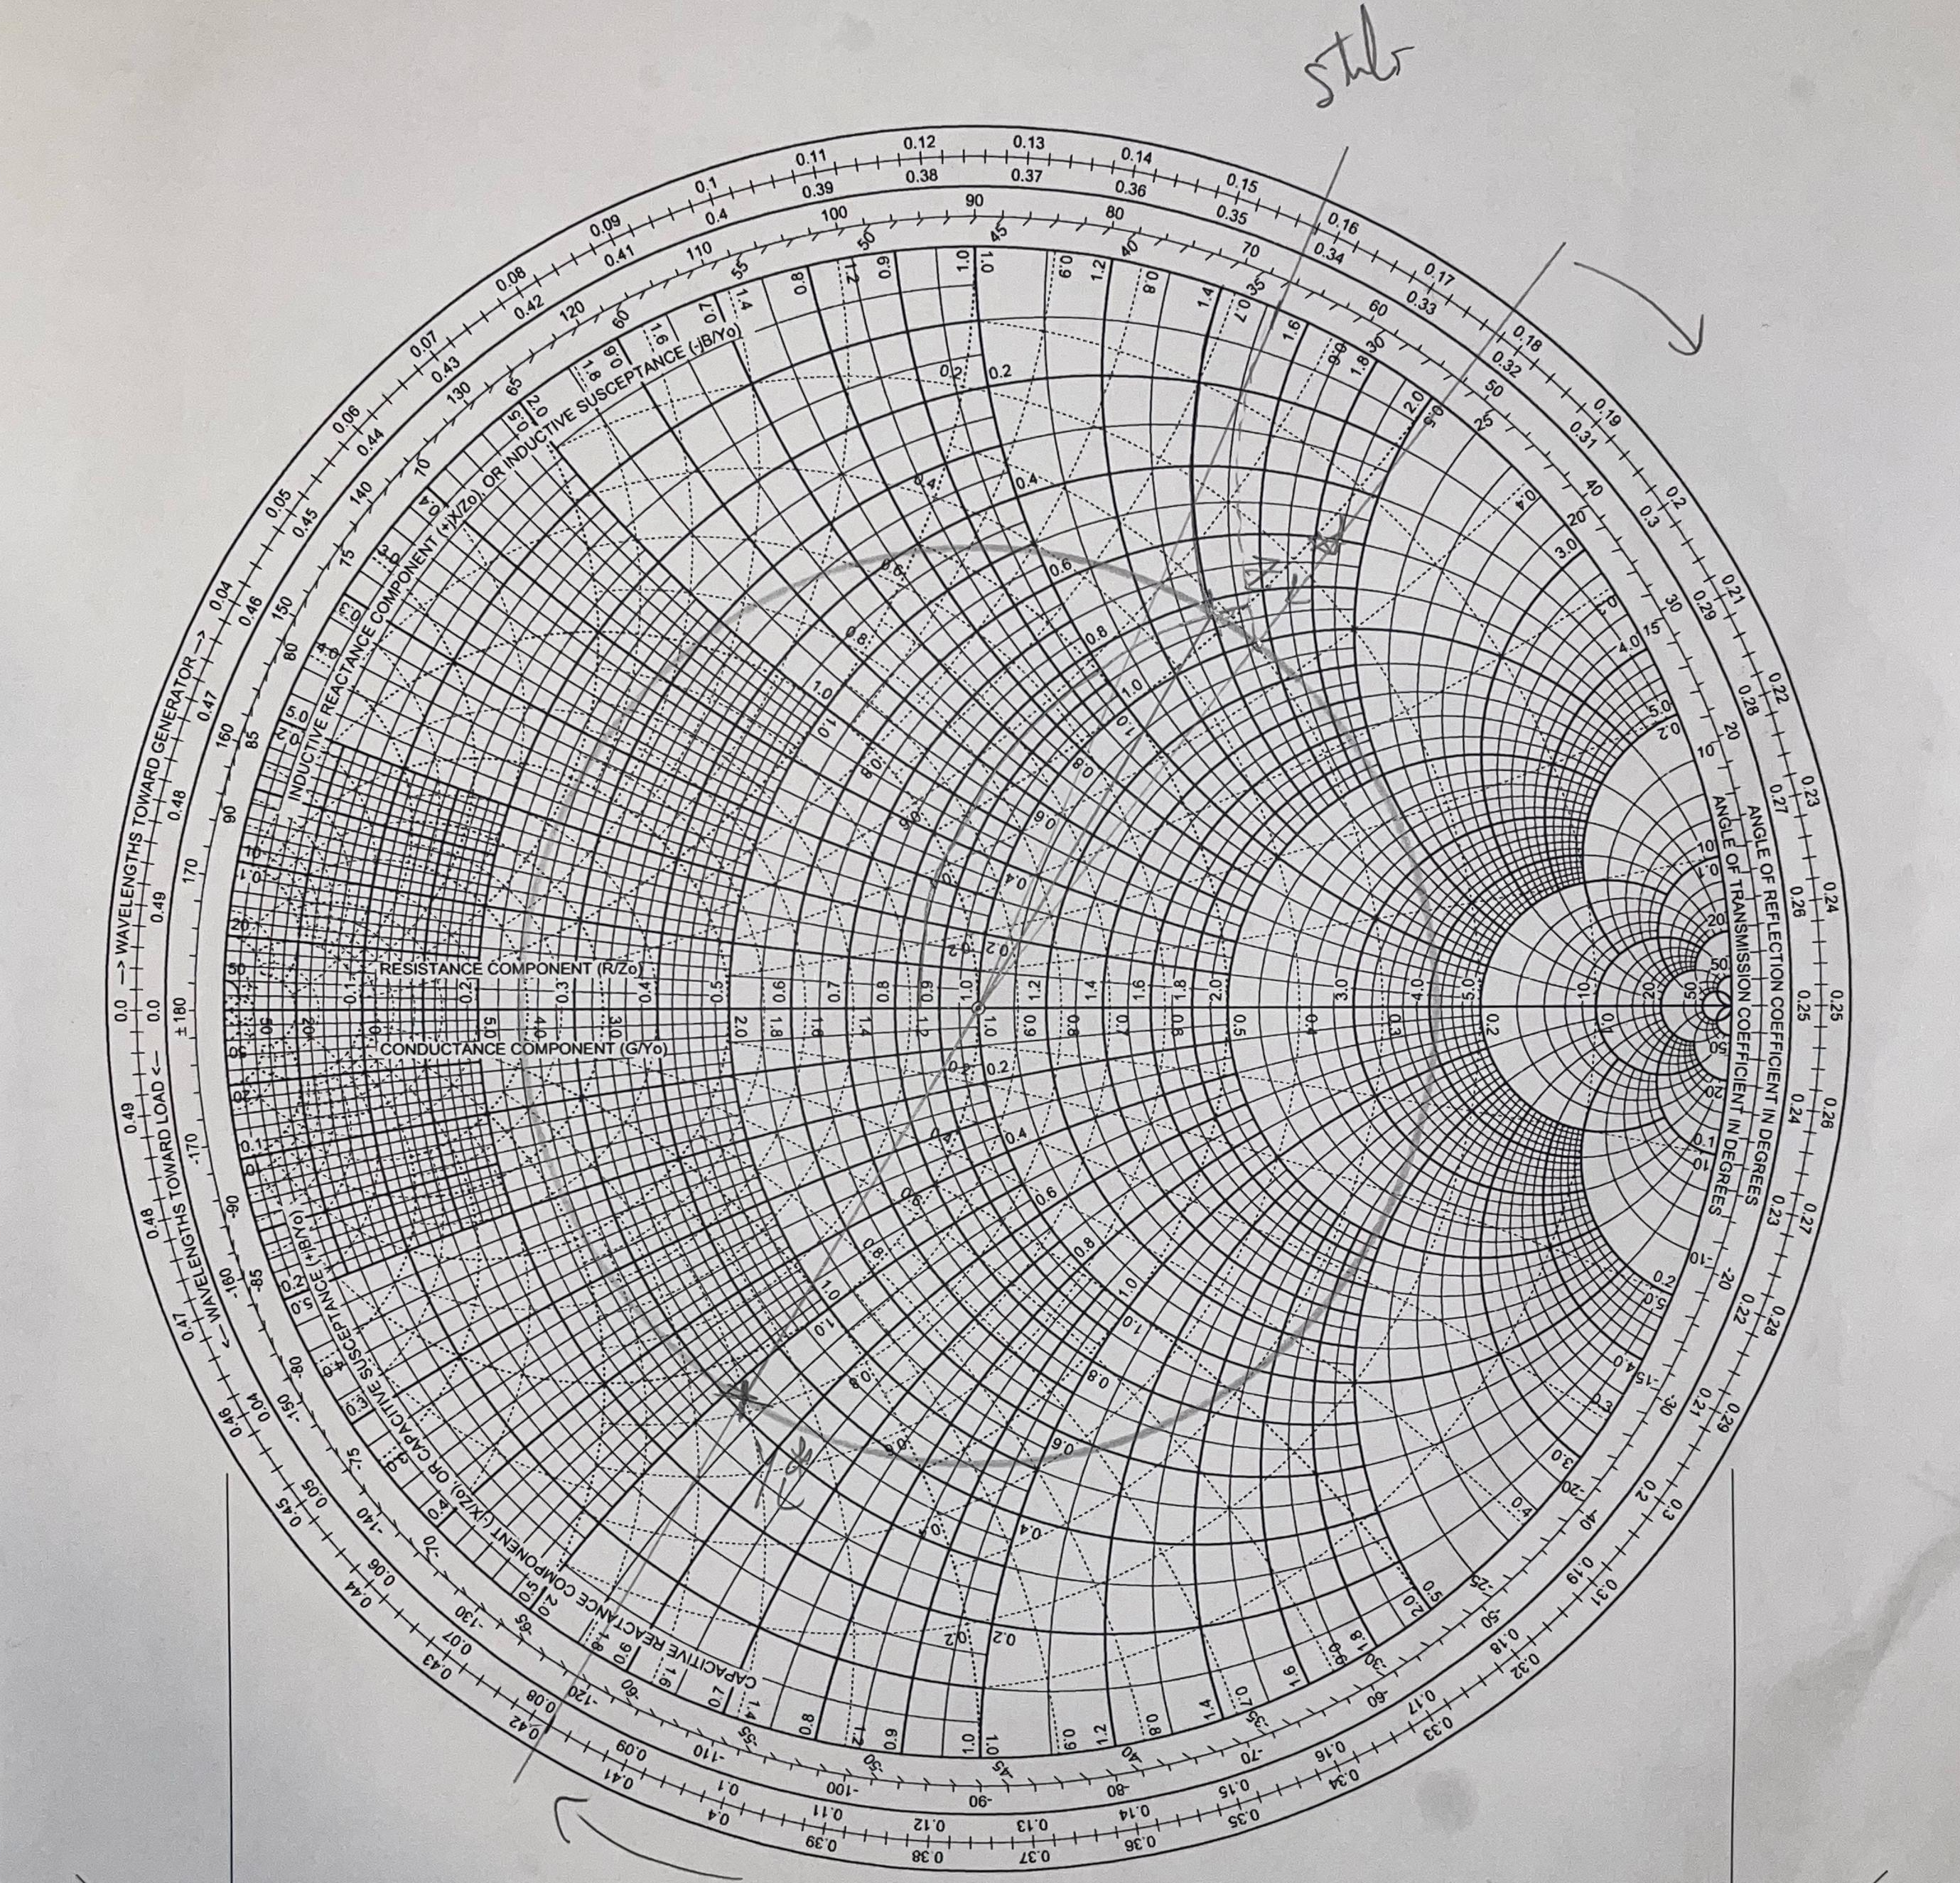
\includegraphics[width=0.5\textwidth]{Images/zl-LS-matching.png}
%     \caption{Matching circuit for input with lines and stubs}
%     \label{fig:zl-line-matching}
% \end{figure}

The adaptation mesh for the output is done with a series line and an open circuit shunt stub.

The final circuit is shown in Figure \ref{fig:MatchingCircuit-line}, where the input and output matching networks are designed using a combination of transmission lines and stubs.

\begin{figure}[H]
    \centering
    \includegraphics[width=1\textwidth]{Images/LS_matching-circuit.png}
    \caption{Matching circuit for input and output with values}
    \label{fig:MatchingCircuit-line}
\end{figure}

%\subsection{Gain and Noise Factor}
